%
% Forecasts.tex
% Forecasts
%
% R for Business Administration
%
% Copyright (C) 2016 Harris Kenny, Brandon DeGolier, Nate Lewis
%
% This document is licensed under the Creative Commons Attribution 4.0
% International Public License (CC BY-SA 4.0)
%

\section{Forecastable Data}
Forecasts are a way to take historical continuous variable data, understand 
trends, and anticipate future outcomes. Forecasts can be used in many ways,
several examples that may be relevant for your organization are outlined below:

\begin{itemize}
 \item Budgeting (dollars spent by department, area, or activity)
 \item Customer support volume (number of emails, calls, or tickets)
 \item Employee headcount (by department, area, or activity)
 \item Website engagement (total visits, unique visits, time spent)
 \item Sales performance (by revenue, units, profits)
 \item Social media engagement (tagged posts, mentions)
\end{itemize}

Let's try exercises using data that could be selected for its business value 
in forecasting.

\section{Viewing Data}
The exercises in this section will use the "freeny" dataset (Quarterly Revenue 
and Explanatory Variable Data for Freeny's) that is included with R. Load this 
data set into R following the instructions outlined in the Installation section
 of this work.

First, view the data by entering the following command in R Script or R 
Console:

\texttt{print(freeny)}

This yields the following results:

\begin{figure}[h!]
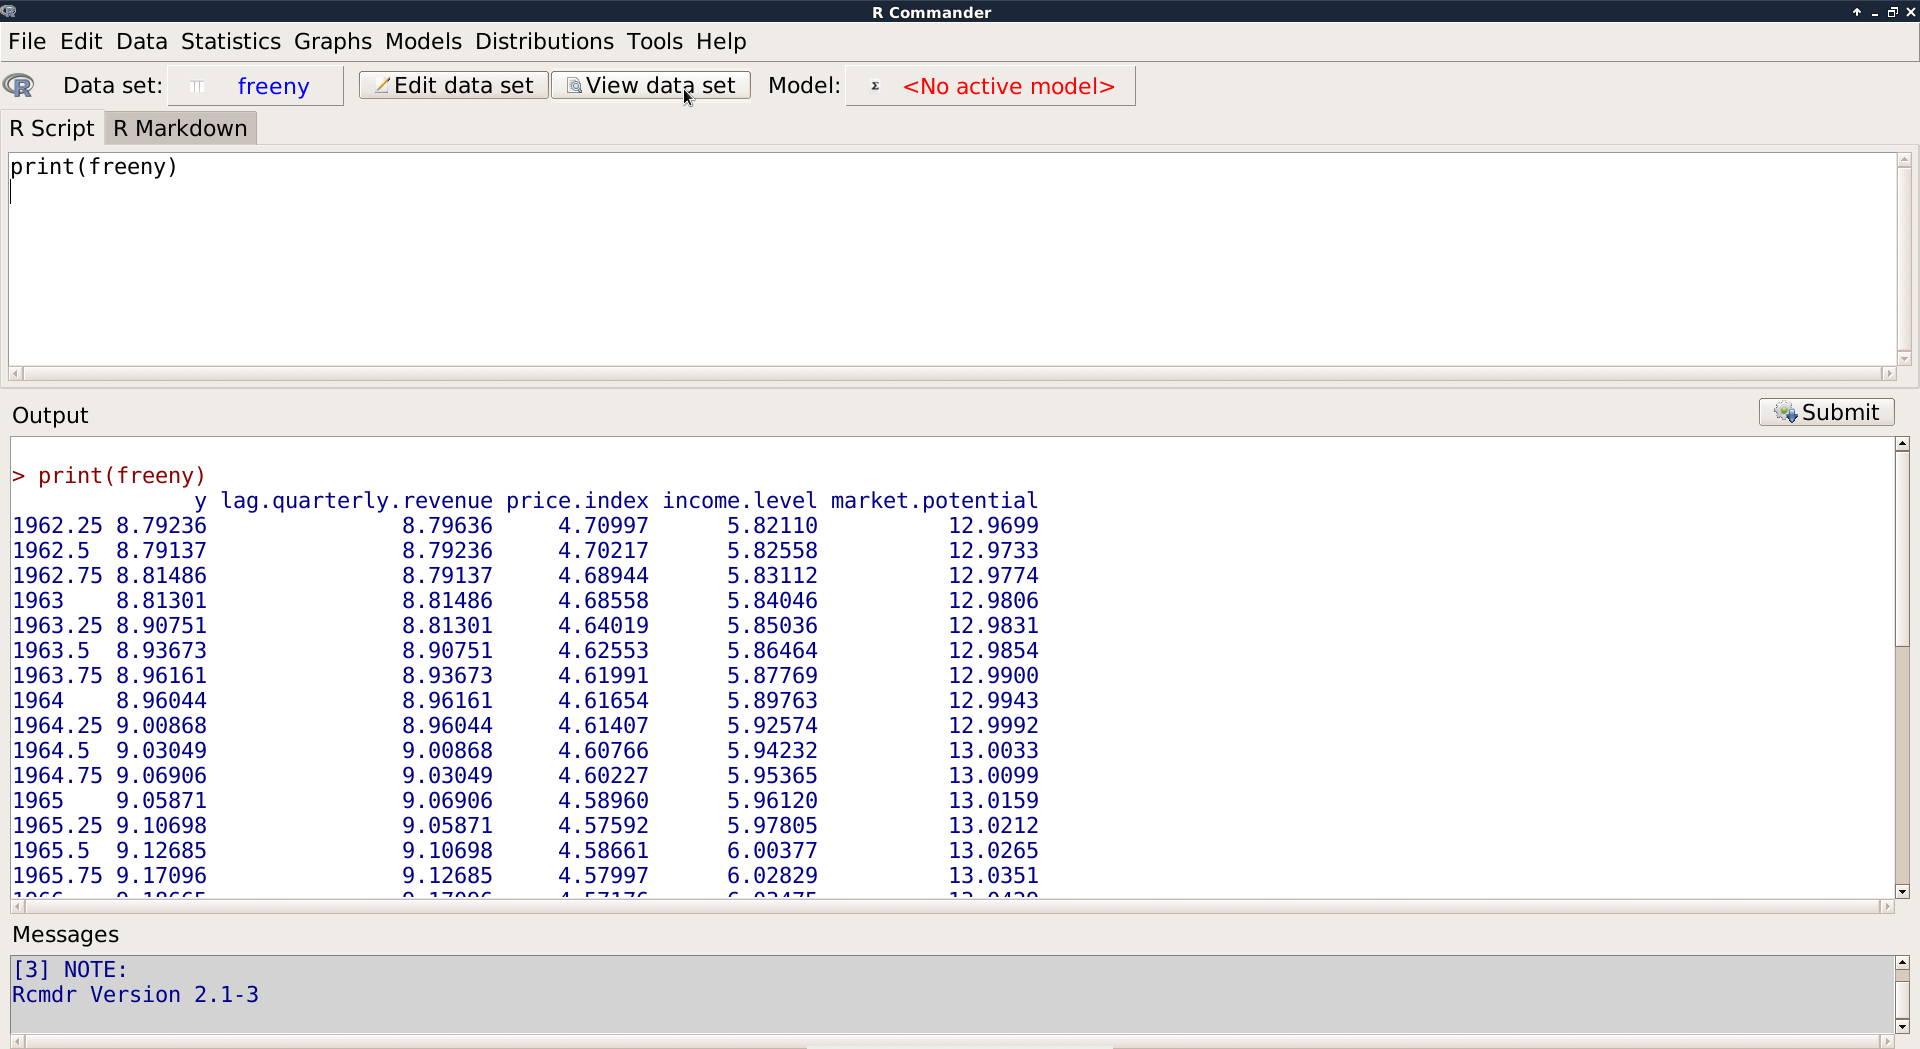
\includegraphics[keepaspectratio=true,height=1.10\textheight,width=1.00\textwidth,angle=0]{print_freeny.png}
 \caption{freeny dataset via R-Commander R Script}
 \label{fig:print_freeny}
\end{figure}

Or, click View data set in R-Commander in the center of the user interface 
window.

This yields the following results:

\begin{figure}[h!]
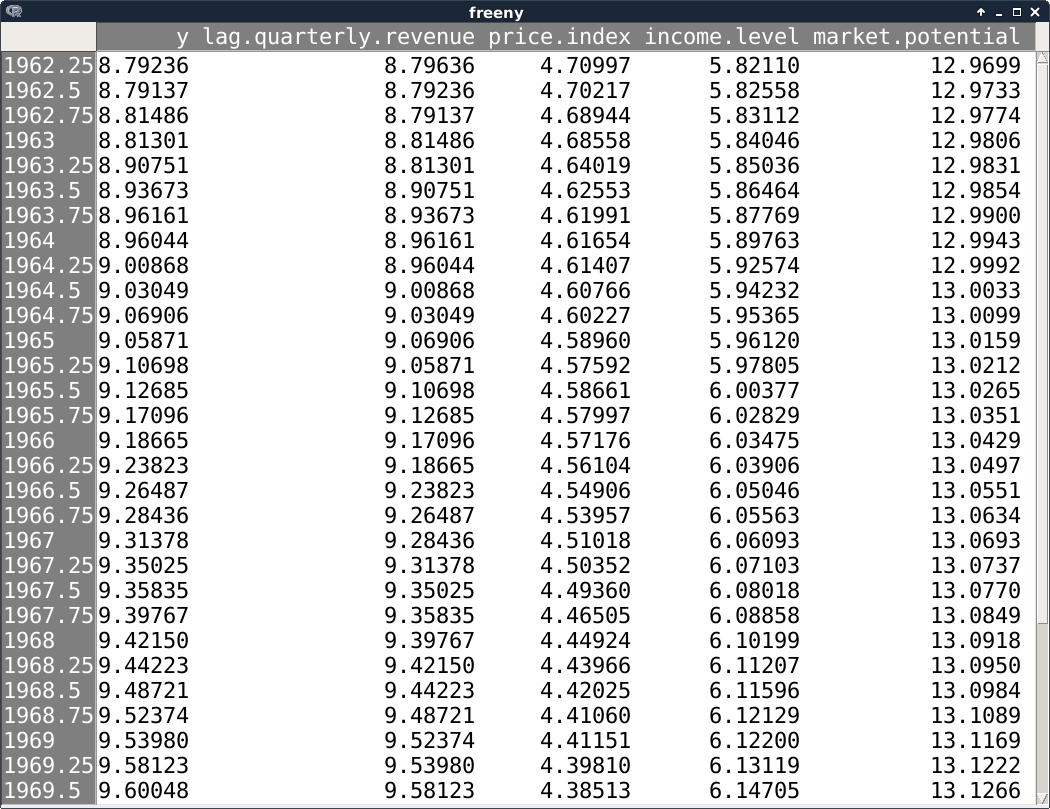
\includegraphics[keepaspectratio=true,height=1.10\textheight,width=1.00\textwidth,angle=0]{view-data-set_freeny.png}
 \caption{freeny dataset via R-Commander GUI}
 \label{fig:view-data-set_freeny}
\end{figure}

To determine how many rows we are dealing with, enter the following command:

\texttt{nrow(freeny)}

This yields the following results:

[1] 39

Meaning there are 39 rows in the dataset. Recall that this is quarterly data. 
39 divided by 4 equals 9.75, meaning this is nine years and three quarters of 
business data. What other variables are included? in the dataset? Enter: 

\texttt{names(freeny)}

\begin{enumerate}
 \item y - 
 \item lag.quarterly.revenue -  
 \item price.index - 
 \item income.level - 
 \item market.potential - 
\end{enumerate}

Since currency is not noted, we can assume that all these values are in the 
same currency, making that one less thing to worry about during our analysis.

\subsection{Averages and Quartiles}
Averages and quartiles are a basic way to capture a snapshot of the data you have collected. Recall there are two types of data (continuous and categorical), so R will generate two types of sets of summary statistics.

Calculate summary statistics by entering the following command:

\texttt{summary(warpbreaks)}

Or, select in R-Commander by going to Statistics > Summaries > Active Dataset. Either way, the result will be generated in the Output window in R-Commander.

This yields the following results:

\begin{figure}[h!]
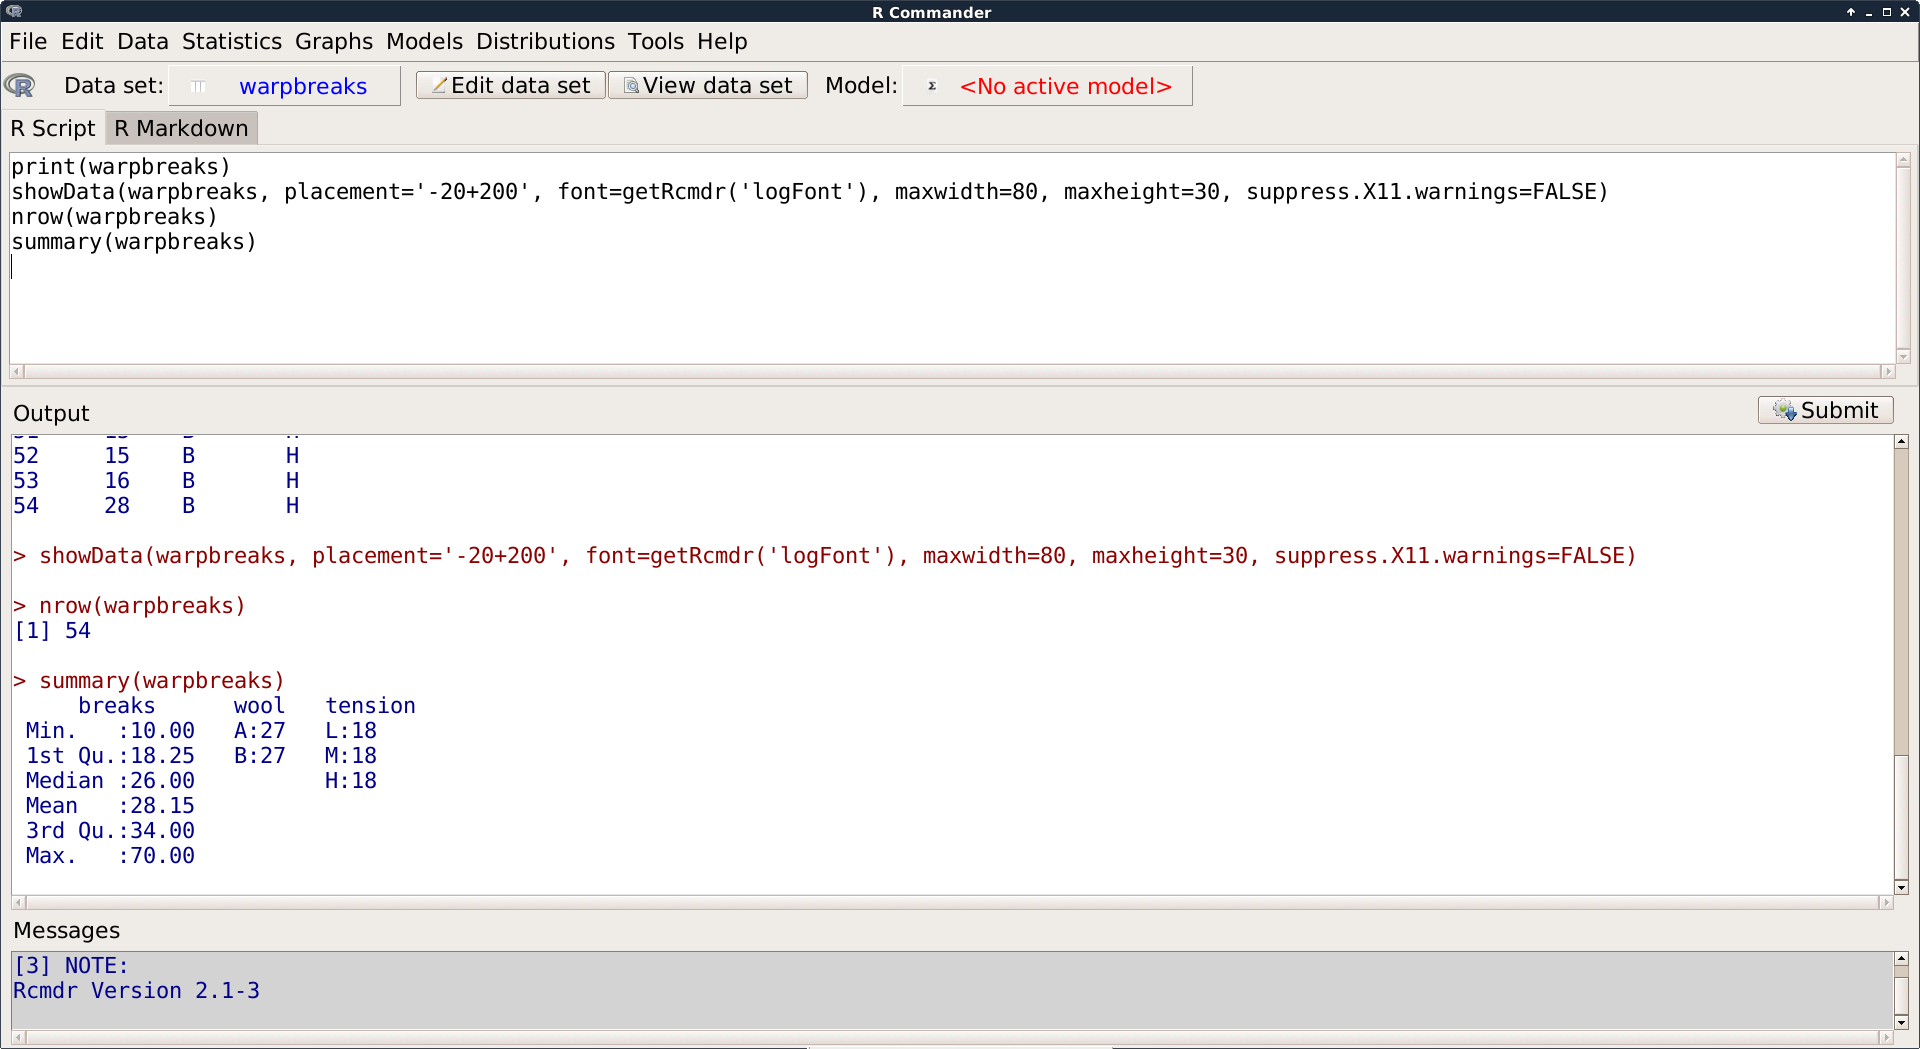
\includegraphics[keepaspectratio=true,height=1.10\textheight,width=1.00\textwidth,angle=0]{summary_warpbreaks.png}
 \caption{warpbreaks dataset summary via R-Commander R Script}
 \label{fig:summary_warpbreaks}
\end{figure}

What is the significance of these results? Let's break them down one-by-one:

\begin{itemize}
 \item Min. - The minimum data point in the dataset. For column "breaks" this number is 10. In other words, of the surveyed samples of yarn, the lowest number of observed breaks in the dataset is 10. Stated differently, the best performing yarn had 10 breaks.
 \item 1st Qu. - The first quartile of data in the dataset. For column "breaks" this number is 18.25. In other words, of the surveyed samples of yarn, the bottom quarter of yarn surveyed had 18.25 breaks.
 \item Median - The median datapoint in the dataset. For column "breaks" this number is 26. In other words, of the surveyed samples of yarn, the middle data point is 26. This is calculated by cross-secting the data to the middle and selecting the single point, or adding the two middle points and dividing by two if the dataset has an even number. Median calculations are especially valuable for datasets that have outliers that may be skewing mean averages (more on this below).
 \item Mean - The mean datapoint for the dataset. For column "breaks" this number is 28.15. This is calculated by summing all of the data points and dividing by the total number (or count) of data points. Mean is what most people are referring to when they use the term average, and is the most common form of average used.
 \item 3rd Qu. - The third quartile of data in the dataset. For column "breaks" this number is 34. In other words, of the surveyed samples of yarn, the top quarter of yarn surveyed had 34 breaks.
 \item Max. - The maximum data point in the dataset. For column "breaks" this number is 70. In other words, of the surveyed samples of yarn, the highest number of observed breaks in the dataset is 70. Stated differently, the worst performing yarn had 70 breaks.
\end{itemize}

What else can we conclude from summary statistics of the "breaks" column? The mean is larger than the median, indicating a possible skew in the data towards the samples of yarn with higher numbers of breaks.

There are two other columns of summary statistics calculated by R: wool and tension. This provides a count summary of these categorical variables. Note that the dataset includes an even number of both types of wool (27 of both A and B). The dataset also includes an even number of all three levels of tension (18 Low, Medium, and High).

There is a third less common measure of average called mode\footnote{In R, mode is more importantly an object characteristic in indicating how the object is stored in memory (e.g. as a number, as a character string, as a function).}, the value that has the highest number of occurrences in the dataset. Calculating mode takes several steps and is not outlined at this time.

% Fill this out later

\section{Generating Metadata from Open Responses}
% Section is incomplete, needs a screen shot to demonstrate how
It is possible to create metadata from open-ended responses in survey questions that you evaluate through statistical techniques.

For example, say a survey asked customers if there is anything your organization could do to better serve them in the future. Have someone from your organization review the responses and generate a list based on topics submitted by customers. 

Next, count each time on appears in the customer responses. This can be done manually or through a formula in spreadsheet software like LibreOffice Calc or Gnumeric.\footnote{Learn more about these projects at \texttt{https://www.libreoffice.org/} and \texttt{http://gnumeric.org/}} This new set of metadata can now be leveraged in proportion tests or other testing methods.